\documentclass[11pt,compress,t,notes=noshow, xcolor=table]{beamer}
\documentclass[11pt,compress,t,notes=noshow, xcolor=table]{beamer}
\usepackage[]{graphicx}\usepackage[]{color}
% maxwidth is the original width if it is less than linewidth
% otherwise use linewidth (to make sure the graphics do not exceed the margin)
\makeatletter
\def\maxwidth{ %
  \ifdim\Gin@nat@width>\linewidth
    \linewidth
  \else
    \Gin@nat@width
  \fi
}
\makeatother

\definecolor{fgcolor}{rgb}{0.345, 0.345, 0.345}
\newcommand{\hlnum}[1]{\textcolor[rgb]{0.686,0.059,0.569}{#1}}%
\newcommand{\hlstr}[1]{\textcolor[rgb]{0.192,0.494,0.8}{#1}}%
\newcommand{\hlcom}[1]{\textcolor[rgb]{0.678,0.584,0.686}{\textit{#1}}}%
\newcommand{\hlopt}[1]{\textcolor[rgb]{0,0,0}{#1}}%
\newcommand{\hlstd}[1]{\textcolor[rgb]{0.345,0.345,0.345}{#1}}%
\newcommand{\hlkwa}[1]{\textcolor[rgb]{0.161,0.373,0.58}{\textbf{#1}}}%
\newcommand{\hlkwb}[1]{\textcolor[rgb]{0.69,0.353,0.396}{#1}}%
\newcommand{\hlkwc}[1]{\textcolor[rgb]{0.333,0.667,0.333}{#1}}%
\newcommand{\hlkwd}[1]{\textcolor[rgb]{0.737,0.353,0.396}{\textbf{#1}}}%
\let\hlipl\hlkwb

\usepackage{framed}
\makeatletter
\newenvironment{kframe}{%
 \def\at@end@of@kframe{}%
 \ifinner\ifhmode%
  \def\at@end@of@kframe{\end{minipage}}%
  \begin{minipage}{\columnwidth}%
 \fi\fi%
 \def\FrameCommand##1{\hskip\@totalleftmargin \hskip-\fboxsep
 \colorbox{shadecolor}{##1}\hskip-\fboxsep
     % There is no \\@totalrightmargin, so:
     \hskip-\linewidth \hskip-\@totalleftmargin \hskip\columnwidth}%
 \MakeFramed {\advance\hsize-\width
   \@totalleftmargin\z@ \linewidth\hsize
   \@setminipage}}%
 {\par\unskip\endMakeFramed%
 \at@end@of@kframe}
\makeatother

\definecolor{shadecolor}{rgb}{.97, .97, .97}
\definecolor{messagecolor}{rgb}{0, 0, 0}
\definecolor{warningcolor}{rgb}{1, 0, 1}
\definecolor{errorcolor}{rgb}{1, 0, 0}
\newenvironment{knitrout}{}{} % an empty environment to be redefined in TeX

\usepackage{alltt}
\newcommand{\SweaveOpts}[1]{}  % do not interfere with LaTeX
\newcommand{\SweaveInput}[1]{} % because they are not real TeX commands
\newcommand{\Sexpr}[1]{}       % will only be parsed by R
\newcommand{\xmark}{\ding{55}}%


\usepackage[english]{babel}
\usepackage[utf8]{inputenc}

\usepackage{dsfont}
\usepackage{verbatim}
\usepackage{amsmath}
\usepackage{amsfonts}
\usepackage{amssymb}
\usepackage{bm}
\usepackage{csquotes}
\usepackage{multirow}
\usepackage{longtable}
\usepackage{booktabs}
\usepackage{enumerate}
\usepackage[absolute,overlay]{textpos}
\usepackage{psfrag}
\usepackage{algorithm}
\usepackage{algpseudocode}
\usepackage{eqnarray}
\usepackage{arydshln}
\usepackage{tabularx}
\usepackage{placeins}
\usepackage{tikz}
\usepackage{setspace}
\usepackage{colortbl}
\usepackage{mathtools}
\usepackage{wrapfig}
\usepackage{bm}
\usepackage{amsmath}
\usepackage{pifont}

\usetikzlibrary{shapes,arrows,automata,positioning,calc,chains,trees, shadows}
\tikzset{
  %Define standard arrow tip
  >=stealth',
  %Define style for boxes
  punkt/.style={
    rectangle,
    rounded corners,
    draw=black, very thick,
    text width=6.5em,
    minimum height=2em,
    text centered},
  % Define arrow style
  pil/.style={
    ->,
    thick,
    shorten <=2pt,
    shorten >=2pt,}
}

\usepackage{subfig}

% Defines macros and environments
\usepackage{../../style/lmu-lecture}


\let\code=\texttt
\let\proglang=\textsf

\setkeys{Gin}{width=0.9\textwidth}

\setbeamertemplate{frametitle}{\expandafter\uppercase\expandafter\insertframetitle}

% This file is included in slides and exercises

% Rarely used fontstyle for R packages, used only in 
% - forests/slides-forests-benchmark.tex
% - exercises/single-exercises/methods_l_1.Rnw
% - slides/cart/attic/slides_extra_trees.Rnw
\newcommand{\pkg}[1]{{\fontseries{b}\selectfont #1}}

% Spacing helpers, used often (mostly in exercises for \dlz)
\newcommand{\lz}{\vspace{0.5cm}} % vertical space (used often in slides)
\newcommand{\dlz}{\vspace{1cm}}  % double vertical space (used often in exercises, never in slides)
\newcommand{\oneliner}[1] % Oneliner for important statements, used e.g. in iml, algods
{\begin{block}{}\begin{center}\begin{Large}#1\end{Large}\end{center}\end{block}}

% Don't know if this is used or needed, remove?
% textcolor that works in mathmode
% https://tex.stackexchange.com/a/261480
% Used e.g. in forests/slides-forests-bagging.tex
% [...] \textcolor{blue}{\tfrac{1}{M}\sum^M_{m} [...]
% \makeatletter
% \renewcommand*{\@textcolor}[3]{%
%   \protect\leavevmode
%   \begingroup
%     \color#1{#2}#3%
%   \endgroup
% }
% \makeatother






% latex-math includes as needed
% dependencies: amsmath, amssymb, dsfont
% math spaces
\ifdefined\N
\renewcommand{\N}{\mathds{N}} % N, naturals
\else \newcommand{\N}{\mathds{N}} \fi
\newcommand{\Z}{\mathds{Z}} % Z, integers
\newcommand{\Q}{\mathds{Q}} % Q, rationals
\newcommand{\R}{\mathds{R}} % R, reals
\ifdefined\C
\renewcommand{\C}{\mathds{C}} % C, complex
\else \newcommand{\C}{\mathds{C}} \fi
\newcommand{\continuous}{\mathcal{C}} % C, space of continuous functions
\newcommand{\M}{\mathcal{M}} % machine numbers
\newcommand{\epsm}{\epsilon_m} % maximum error

% counting / finite sets
\newcommand{\setzo}{\{0, 1\}} % set 0, 1
\newcommand{\setmp}{\{-1, +1\}} % set -1, 1
\newcommand{\unitint}{[0, 1]} % unit interval

% basic math stuff
\newcommand{\xt}{\tilde x} % x tilde
\newcommand{\argmin}{\mathop{\mathrm{arg\,min}}} % argmin
\newcommand{\argmax}{\mathop{\mathrm{arg\,max}}} % argmax
\newcommand{\argminlim}{\argmin\limits} % argmin with limits
\newcommand{\argmaxlim}{\argmax\limits} % argmax with limits
\newcommand{\sign}{\operatorname{sign}} % sign, signum
\newcommand{\I}{\mathbb{I}} % I, indicator
\newcommand{\order}{\mathcal{O}} % O, order
\newcommand{\bigO}{\mathcal{O}} % Big-O Landau
\newcommand{\littleo}{{o}} % Little-o Landau
\newcommand{\pd}[2]{\frac{\partial{#1}}{\partial #2}} % partial derivative
\newcommand{\floorlr}[1]{\left\lfloor #1 \right\rfloor} % floor
\newcommand{\ceillr}[1]{\left\lceil #1 \right\rceil} % ceiling
\newcommand{\indep}{\perp \!\!\! \perp} % independence symbol

% sums and products
\newcommand{\sumin}{\sum\limits_{i=1}^n} % summation from i=1 to n
\newcommand{\sumim}{\sum\limits_{i=1}^m} % summation from i=1 to m
\newcommand{\sumjn}{\sum\limits_{j=1}^n} % summation from j=1 to p
\newcommand{\sumjp}{\sum\limits_{j=1}^p} % summation from j=1 to p
\newcommand{\sumik}{\sum\limits_{i=1}^k} % summation from i=1 to k
\newcommand{\sumkg}{\sum\limits_{k=1}^g} % summation from k=1 to g
\newcommand{\sumjg}{\sum\limits_{j=1}^g} % summation from j=1 to g
\newcommand{\summM}{\sum\limits_{m=1}^M} % summation from m=1 to M
\newcommand{\meanin}{\frac{1}{n} \sum\limits_{i=1}^n} % mean from i=1 to n
\newcommand{\meanim}{\frac{1}{m} \sum\limits_{i=1}^m} % mean from i=1 to n
\newcommand{\meankg}{\frac{1}{g} \sum\limits_{k=1}^g} % mean from k=1 to g
\newcommand{\meanmM}{\frac{1}{M} \sum\limits_{m=1}^M} % mean from m=1 to M
\newcommand{\prodin}{\prod\limits_{i=1}^n} % product from i=1 to n
\newcommand{\prodkg}{\prod\limits_{k=1}^g} % product from k=1 to g
\newcommand{\prodjp}{\prod\limits_{j=1}^p} % product from j=1 to p

% linear algebra
\newcommand{\one}{\bm{1}} % 1, unitvector
\newcommand{\zero}{\mathbf{0}} % 0-vector
\newcommand{\id}{\bm{I}} % I, identity
\newcommand{\diag}{\operatorname{diag}} % diag, diagonal
\newcommand{\trace}{\operatorname{tr}} % tr, trace
\newcommand{\spn}{\operatorname{span}} % span
\newcommand{\scp}[2]{\left\langle #1, #2 \right\rangle} % <.,.>, scalarproduct
\newcommand{\mat}[1]{\begin{pmatrix} #1 \end{pmatrix}} % short pmatrix command
\newcommand{\Amat}{\mathbf{A}} % matrix A
\newcommand{\Deltab}{\mathbf{\Delta}} % error term for vectors

% basic probability + stats
\renewcommand{\P}{\mathds{P}} % P, probability
\newcommand{\E}{\mathds{E}} % E, expectation
\newcommand{\var}{\mathsf{Var}} % Var, variance
\newcommand{\cov}{\mathsf{Cov}} % Cov, covariance
\newcommand{\corr}{\mathsf{Corr}} % Corr, correlation
\newcommand{\normal}{\mathcal{N}} % N of the normal distribution
\newcommand{\iid}{\overset{i.i.d}{\sim}} % dist with i.i.d superscript
\newcommand{\distas}[1]{\overset{#1}{\sim}} % ... is distributed as ...

% machine learning
\newcommand{\Xspace}{\mathcal{X}} % X, input space
\newcommand{\Yspace}{\mathcal{Y}} % Y, output space
\newcommand{\Zspace}{\mathcal{Z}} % Z, space of sampled datapoints
\newcommand{\nset}{\{1, \ldots, n\}} % set from 1 to n
\newcommand{\pset}{\{1, \ldots, p\}} % set from 1 to p
\newcommand{\gset}{\{1, \ldots, g\}} % set from 1 to g
\newcommand{\Pxy}{\mathbb{P}_{xy}} % P_xy
\newcommand{\Exy}{\mathbb{E}_{xy}} % E_xy: Expectation over random variables xy
\newcommand{\xv}{\mathbf{x}} % vector x (bold)
\newcommand{\xtil}{\tilde{\mathbf{x}}} % vector x-tilde (bold)
\newcommand{\yv}{\mathbf{y}} % vector y (bold)
\newcommand{\xy}{(\xv, y)} % observation (x, y)
\newcommand{\xvec}{\left(x_1, \ldots, x_p\right)^\top} % (x1, ..., xp)
\newcommand{\Xmat}{\mathbf{X}} % Design matrix
\newcommand{\allDatasets}{\mathds{D}} % The set of all datasets
\newcommand{\allDatasetsn}{\mathds{D}_n}  % The set of all datasets of size n
\newcommand{\D}{\mathcal{D}} % D, data
\newcommand{\Dn}{\D_n} % D_n, data of size n
\newcommand{\Dtrain}{\mathcal{D}_{\text{train}}} % D_train, training set
\newcommand{\Dtest}{\mathcal{D}_{\text{test}}} % D_test, test set
\newcommand{\xyi}[1][i]{\left(\xv^{(#1)}, y^{(#1)}\right)} % (x^i, y^i), i-th observation
\newcommand{\Dset}{\left( \xyi[1], \ldots, \xyi[n]\right)} % {(x1,y1)), ..., (xn,yn)}, data
\newcommand{\defAllDatasetsn}{(\Xspace \times \Yspace)^n} % Def. of the set of all datasets of size n
\newcommand{\defAllDatasets}{\bigcup_{n \in \N}(\Xspace \times \Yspace)^n} % Def. of the set of all datasets
\newcommand{\xdat}{\left\{ \xv^{(1)}, \ldots, \xv^{(n)}\right\}} % {x1, ..., xn}, input data
\newcommand{\ydat}{\left\{ \yv^{(1)}, \ldots, \yv^{(n)}\right\}} % {y1, ..., yn}, input data
\newcommand{\yvec}{\left(y^{(1)}, \hdots, y^{(n)}\right)^\top} % (y1, ..., yn), vector of outcomes
\newcommand{\greekxi}{\xi} % Greek letter xi
\renewcommand{\xi}[1][i]{\xv^{(#1)}} % x^i, i-th observed value of x
\newcommand{\yi}[1][i]{y^{(#1)}} % y^i, i-th observed value of y
\newcommand{\xivec}{\left(x^{(i)}_1, \ldots, x^{(i)}_p\right)^\top} % (x1^i, ..., xp^i), i-th observation vector
\newcommand{\xj}{\xv_j} % x_j, j-th feature
\newcommand{\xjvec}{\left(x^{(1)}_j, \ldots, x^{(n)}_j\right)^\top} % (x^1_j, ..., x^n_j), j-th feature vector
\newcommand{\phiv}{\mathbf{\phi}} % Basis transformation function phi
\newcommand{\phixi}{\mathbf{\phi}^{(i)}} % Basis transformation of xi: phi^i := phi(xi)

%%%%%% ml - models general
\newcommand{\lamv}{\bm{\lambda}} % lambda vector, hyperconfiguration vector
\newcommand{\Lam}{\bm{\Lambda}}	 % Lambda, space of all hpos
% Inducer / Inducing algorithm
\newcommand{\preimageInducer}{\left(\defAllDatasets\right)\times\Lam} % Set of all datasets times the hyperparameter space
\newcommand{\preimageInducerShort}{\allDatasets\times\Lam} % Set of all datasets times the hyperparameter space
% Inducer / Inducing algorithm
\newcommand{\ind}{\mathcal{I}} % Inducer, inducing algorithm, learning algorithm

% continuous prediction function f
\newcommand{\ftrue}{f_{\text{true}}}  % True underlying function (if a statistical model is assumed)
\newcommand{\ftruex}{\ftrue(\xv)} % True underlying function (if a statistical model is assumed)
\newcommand{\fx}{f(\xv)} % f(x), continuous prediction function
\newcommand{\fdomains}{f: \Xspace \rightarrow \R^g} % f with domain and co-domain
\newcommand{\Hspace}{\mathcal{H}} % hypothesis space where f is from
\newcommand{\fbayes}{f^{\ast}} % Bayes-optimal model
\newcommand{\fxbayes}{f^{\ast}(\xv)} % Bayes-optimal model
\newcommand{\fkx}[1][k]{f_{#1}(\xv)} % f_j(x), discriminant component function
\newcommand{\fh}{\hat{f}} % f hat, estimated prediction function
\newcommand{\fxh}{\fh(\xv)} % fhat(x)
\newcommand{\fxt}{f(\xv ~|~ \thetav)} % f(x | theta)
\newcommand{\fxi}{f\left(\xv^{(i)}\right)} % f(x^(i))
\newcommand{\fxih}{\hat{f}\left(\xv^{(i)}\right)} % f(x^(i))
\newcommand{\fxit}{f\left(\xv^{(i)} ~|~ \thetav\right)} % f(x^(i) | theta)
\newcommand{\fhD}{\fh_{\D}} % fhat_D, estimate of f based on D
\newcommand{\fhDtrain}{\fh_{\Dtrain}} % fhat_Dtrain, estimate of f based on D
\newcommand{\fhDnlam}{\fh_{\Dn, \lamv}} %model learned on Dn with hp lambda
\newcommand{\fhDlam}{\fh_{\D, \lamv}} %model learned on D with hp lambda
\newcommand{\fhDnlams}{\fh_{\Dn, \lamv^\ast}} %model learned on Dn with optimal hp lambda
\newcommand{\fhDlams}{\fh_{\D, \lamv^\ast}} %model learned on D with optimal hp lambda

% discrete prediction function h
\newcommand{\hx}{h(\xv)} % h(x), discrete prediction function
\newcommand{\hh}{\hat{h}} % h hat
\newcommand{\hxh}{\hat{h}(\xv)} % hhat(x)
\newcommand{\hxt}{h(\xv | \thetav)} % h(x | theta)
\newcommand{\hxi}{h\left(\xi\right)} % h(x^(i))
\newcommand{\hxit}{h\left(\xi ~|~ \thetav\right)} % h(x^(i) | theta)
\newcommand{\hbayes}{h^{\ast}} % Bayes-optimal classification model
\newcommand{\hxbayes}{h^{\ast}(\xv)} % Bayes-optimal classification model

% yhat
\newcommand{\yh}{\hat{y}} % yhat for prediction of target
\newcommand{\yih}{\hat{y}^{(i)}} % yhat^(i) for prediction of ith targiet
\newcommand{\resi}{\yi- \yih}

% theta
\newcommand{\thetah}{\hat{\theta}} % theta hat
\newcommand{\thetav}{\bm{\theta}} % theta vector
\newcommand{\thetavh}{\bm{\hat\theta}} % theta vector hat
\newcommand{\thetat}[1][t]{\thetav^{[#1]}} % theta^[t] in optimization
\newcommand{\thetatn}[1][t]{\thetav^{[#1 +1]}} % theta^[t+1] in optimization
\newcommand{\thetahDnlam}{\thetavh_{\Dn, \lamv}} %theta learned on Dn with hp lambda
\newcommand{\thetahDlam}{\thetavh_{\D, \lamv}} %theta learned on D with hp lambda
\newcommand{\mint}{\min_{\thetav \in \Theta}} % min problem theta
\newcommand{\argmint}{\argmin_{\thetav \in \Theta}} % argmin theta

% densities + probabilities
% pdf of x
\newcommand{\pdf}{p} % p
\newcommand{\pdfx}{p(\xv)} % p(x)
\newcommand{\pixt}{\pi(\xv~|~ \thetav)} % pi(x|theta), pdf of x given theta
\newcommand{\pixit}[1][i]{\pi\left(\xi[#1] ~|~ \thetav\right)} % pi(x^i|theta), pdf of x given theta
\newcommand{\pixii}[1][i]{\pi\left(\xi[#1]\right)} % pi(x^i), pdf of i-th x

% pdf of (x, y)
\newcommand{\pdfxy}{p(\xv,y)} % p(x, y)
\newcommand{\pdfxyt}{p(\xv, y ~|~ \thetav)} % p(x, y | theta)
\newcommand{\pdfxyit}{p\left(\xi, \yi ~|~ \thetav\right)} % p(x^(i), y^(i) | theta)

% pdf of x given y
\newcommand{\pdfxyk}[1][k]{p(\xv | y= #1)} % p(x | y = k)
\newcommand{\lpdfxyk}[1][k]{\log p(\xv | y= #1)} % log p(x | y = k)
\newcommand{\pdfxiyk}[1][k]{p\left(\xi | y= #1 \right)} % p(x^i | y = k)

% prior probabilities
\newcommand{\pik}[1][k]{\pi_{#1}} % pi_k, prior
\newcommand{\lpik}[1][k]{\log \pi_{#1}} % log pi_k, log of the prior
\newcommand{\pit}{\pi(\thetav)} % Prior probability of parameter theta

% posterior probabilities
\newcommand{\post}{\P(y = 1 ~|~ \xv)} % P(y = 1 | x), post. prob for y=1
\newcommand{\postk}[1][k]{\P(y = #1 ~|~ \xv)} % P(y = k | y), post. prob for y=k
\newcommand{\pidomains}{\pi: \Xspace \rightarrow \unitint} % pi with domain and co-domain
\newcommand{\pibayes}{\pi^{\ast}} % Bayes-optimal classification model
\newcommand{\pixbayes}{\pi^{\ast}(\xv)} % Bayes-optimal classification model
\newcommand{\pix}{\pi(\xv)} % pi(x), P(y = 1 | x)
\newcommand{\piv}{\bm{\pi}} % pi, bold, as vector
\newcommand{\pikx}[1][k]{\pi_{#1}(\xv)} % pi_k(x), P(y = k | x)
\newcommand{\pikxt}[1][k]{\pi_{#1}(\xv ~|~ \thetav)} % pi_k(x | theta), P(y = k | x, theta)
\newcommand{\pixh}{\hat \pi(\xv)} % pi(x) hat, P(y = 1 | x) hat
\newcommand{\pikxh}[1][k]{\hat \pi_{#1}(\xv)} % pi_k(x) hat, P(y = k | x) hat
\newcommand{\pixih}{\hat \pi(\xi)} % pi(x^(i)) with hat
\newcommand{\pikxih}[1][k]{\hat \pi_{#1}(\xi)} % pi_k(x^(i)) with hat
\newcommand{\pdfygxt}{p(y ~|~\xv, \thetav)} % p(y | x, theta)
\newcommand{\pdfyigxit}{p\left(\yi ~|~\xi, \thetav\right)} % p(y^i |x^i, theta)
\newcommand{\lpdfygxt}{\log \pdfygxt } % log p(y | x, theta)
\newcommand{\lpdfyigxit}{\log \pdfyigxit} % log p(y^i |x^i, theta)

% probababilistic
\newcommand{\bayesrulek}[1][k]{\frac{\P(\xv | y= #1) \P(y= #1)}{\P(\xv)}} % Bayes rule
\newcommand{\muk}{\bm{\mu_k}} % mean vector of class-k Gaussian (discr analysis)

% residual and margin
\newcommand{\eps}{\epsilon} % residual, stochastic
\newcommand{\epsv}{\bm{\epsilon}} % residual, stochastic, as vector
\newcommand{\epsi}{\epsilon^{(i)}} % epsilon^i, residual, stochastic
\newcommand{\epsh}{\hat{\epsilon}} % residual, estimated
\newcommand{\epsvh}{\hat{\epsv}} % residual, estimated, vector
\newcommand{\yf}{y \fx} % y f(x), margin
\newcommand{\yfi}{\yi \fxi} % y^i f(x^i), margin
\newcommand{\Sigmah}{\hat \Sigma} % estimated covariance matrix
\newcommand{\Sigmahj}{\hat \Sigma_j} % estimated covariance matrix for the j-th class

% ml - loss, risk, likelihood
\newcommand{\Lyf}{L\left(y, f\right)} % L(y, f), loss function
\newcommand{\Lypi}{L\left(y, \pi\right)} % L(y, pi), loss function
\newcommand{\Lxy}{L\left(y, \fx\right)} % L(y, f(x)), loss function
\newcommand{\Lxyi}{L\left(\yi, \fxi\right)} % loss of observation
\newcommand{\Lxyt}{L\left(y, \fxt\right)} % loss with f parameterized
\newcommand{\Lxyit}{L\left(\yi, \fxit\right)} % loss of observation with f parameterized
\newcommand{\Lxym}{L\left(\yi, f\left(\bm{\tilde{x}}^{(i)} ~|~ \thetav\right)\right)} % loss of observation with f parameterized
\newcommand{\Lpixy}{L\left(y, \pix\right)} % loss in classification
\newcommand{\Lpiy}{L\left(y, \pi\right)} % loss in classification
\newcommand{\Lpiv}{L\left(y, \piv\right)} % loss in classification
\newcommand{\Lpixyi}{L\left(\yi, \pixii\right)} % loss of observation in classification
\newcommand{\Lpixyt}{L\left(y, \pixt\right)} % loss with pi parameterized
\newcommand{\Lpixyit}{L\left(\yi, \pixit\right)} % loss of observation with pi parameterized
\newcommand{\Lhy}{L\left(y, h\right)} % L(y, h), loss function on discrete classes
\newcommand{\Lhxy}{L\left(y, \hx\right)} % L(y, h(x)), loss function on discrete classes
\newcommand{\Lr}{L\left(r\right)} % L(r), loss defined on residual (reg) / margin (classif)
\newcommand{\lone}{|y - \fx|} % L1 loss
\newcommand{\ltwo}{\left(y - \fx\right)^2} % L2 loss
\newcommand{\lbernoullimp}{\ln(1 + \exp(-y \cdot \fx))} % Bernoulli loss for -1, +1 encoding
\newcommand{\lbernoullizo}{- y \cdot \fx + \log(1 + \exp(\fx))} % Bernoulli loss for 0, 1 encoding
\newcommand{\lcrossent}{- y \log \left(\pix\right) - (1 - y) \log \left(1 - \pix\right)} % cross-entropy loss
\newcommand{\lbrier}{\left(\pix - y \right)^2} % Brier score
\newcommand{\risk}{\mathcal{R}} % R, risk
\newcommand{\riskbayes}{\mathcal{R}^\ast}
\newcommand{\riskf}{\risk(f)} % R(f), risk
\newcommand{\riskdef}{\E_{y|\xv}\left(\Lxy \right)} % risk def (expected loss)
\newcommand{\riskt}{\mathcal{R}(\thetav)} % R(theta), risk
\newcommand{\riske}{\mathcal{R}_{\text{emp}}} % R_emp, empirical risk w/o factor 1 / n
\newcommand{\riskeb}{\bar{\mathcal{R}}_{\text{emp}}} % R_emp, empirical risk w/ factor 1 / n
\newcommand{\riskef}{\riske(f)} % R_emp(f)
\newcommand{\risket}{\mathcal{R}_{\text{emp}}(\thetav)} % R_emp(theta)
\newcommand{\riskr}{\mathcal{R}_{\text{reg}}} % R_reg, regularized risk
\newcommand{\riskrt}{\mathcal{R}_{\text{reg}}(\thetav)} % R_reg(theta)
\newcommand{\riskrf}{\riskr(f)} % R_reg(f)
\newcommand{\riskrth}{\hat{\mathcal{R}}_{\text{reg}}(\thetav)} % hat R_reg(theta)
\newcommand{\risketh}{\hat{\mathcal{R}}_{\text{emp}}(\thetav)} % hat R_emp(theta)
\newcommand{\LL}{\mathcal{L}} % L, likelihood
\newcommand{\LLt}{\mathcal{L}(\thetav)} % L(theta), likelihood
\newcommand{\LLtx}{\mathcal{L}(\thetav | \xv)} % L(theta|x), likelihood
\newcommand{\logl}{\ell} % l, log-likelihood
\newcommand{\loglt}{\logl(\thetav)} % l(theta), log-likelihood
\newcommand{\logltx}{\logl(\thetav | \xv)} % l(theta|x), log-likelihood
\newcommand{\errtrain}{\text{err}_{\text{train}}} % training error
\newcommand{\errtest}{\text{err}_{\text{test}}} % test error
\newcommand{\errexp}{\overline{\text{err}_{\text{test}}}} % avg training error

% lm
\newcommand{\thx}{\thetav^\top \xv} % linear model
\newcommand{\olsest}{(\Xmat^\top \Xmat)^{-1} \Xmat^\top \yv} % OLS estimator in LM


% Lecture title always has to be there
\title{Algorithms and Data Structures}

\begin{document}

\titlemeta{% Chunk title (example: CART, Forests, Boosting, ...), can be empty
Encoding
}{% Lecture title
Machine numbers for $\R$
}{% Relative path to title page image: Can be empty but must not start with slides/
}{% Learning goals, wrapped inside itemize environment
  \item IEEE745
  \item Floating point number
  \item Distance
}




\begin{vbframe}{Reals on a Machine}
\begin{itemize}
\item Floating point numbers on a machine don't correspond to $\R$ in a mathematical sense.
  They are merely an approximation.
\item Because there is only a finite number of machine numbers,
  there are no arbitrarily small or large numbers and also no arbitrarily close numbers.
\item A finite subset of the real numbers cannot be closed w.r.t. rational operations (+,-,*,:) %$^*$
\end{itemize}

\lz

We would like to have:
\begin{itemize}
  \item Operations as similar as possible to those in $\R$,
  \item fast and easy implementation on digital computers.
\end{itemize}
\end{vbframe}


\begin{vbframe}{Machine numbers for $\R$ : IEEE 754}

IEEE (\textbf{I}nstitute of \textbf{E}lectrical and \textbf{E}lectronics \textbf{E}ngineers) 754 defines standard representations for floating point numbers in computers.

\lz

Characterized by:
\begin{itemize}
\item Sign bit $S\in\{-1, +1\}$
\item Base $b>$1, common are $2$, $8$, $10$ and $16$ (usually 2)
\item Mantissa of length $m$, the significant bits / digits
\item Smallest and largest exponent $e_{\min}<0$ and $e_{\max}>0$
\item Mantissa, exponent and $S$ are coded as bits $u_i$
\end{itemize}

\lz

Representation:
$$
x = S \cdot b^e \cdot (1 + \sumim u_{i} b^{-i}) %\quad \mbox{or} \quad \mbox (\pm, e, (u_1,\dots,u_m))
$$
Thus: a sign bit, an exponent and the significant digits (binary coded with mantissa bits $u_i, i = 1,..., m$).
%In implementations are usually $b = 2$ and the exponent is a binary coded integer.
\end{vbframe}


\begin{vbframe}{IEEE 754}

Single precision, 32 bit:
\begin{itemize}
  \item $b = 2$; $u_{32}$: sign bit
  \item $e$ is $8$ bits $u_{24}, ..., u_{31}$ (excess coding with bias $127$)
  \item $m = 23$, the first 23 bits are used for the mantissa.
\end{itemize}

\begin{center}
\begin{tabular}{l}
  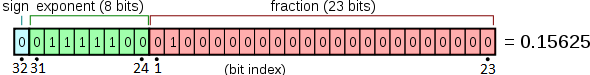
\includegraphics{figure_man/32bit_new} \\[0.15cm]
\end{tabular}
{\scriptsize
Source: \url{https://en.wikipedia.org/wiki/Single-precision_floating-point_format}\\\
Converter: \url{https://www.h-schmidt.net/FloatConverter/IEEE754.html}
}
\end{center}

Example:
\begin{itemize}
  \item sign bit $u_{32} = 0 \Rightarrow S = +1$
  \item $e = \sum_{i=1}^{8} u_{i+23} 2^{i-1} - 127 = 2^2 + 2^3+ 2^4+ 2^5 + 2^6 - 127 = -3$
  \item mantissa bits: $u_2 = 1, u_1=u_3=...=u_{23}=0$
\end{itemize}


$\Rightarrow x = S \cdot b^e \cdot (1 + \sum_{i=1}^{23} u_{i} b^{-i}) = 1 \cdot 2^{-3} \cdot (1 + 2^{-2}) = 0.15625$

\framebreak

Double precision, 64 bit:
\begin{itemize}
  \item $b = 2$; $u_{64}$: sign bit
  \item $e$ is $11$ bits $u_{53}, ..., u_{63}$ (excess coding with bias $1023$)
  \item $m = 52$
\end{itemize}


% \begin{footnotesize}
% \begin{table}
%     \begin{tabular}{lll}
%     ~                                & genauer Wert  & wiss. Schreibweise\\
%      kleinste Zahl (normalisiert)    & $2^{-1022}$    & $2 \cdot 10^{-308}$                                       \\
%     kleinste Zahl (denormalisiert)   & $2^{-1022} \cdot 2^{-52}$ &   $5 \cdot 10^{-324}$      \\
%      größte Zahl    & $2^{1023} \cdot (1+\sum_{i=1}^{52} 2^{-i})$   & $2 \cdot 10^{308}$\\
%     \end{tabular}
% \end{table}
% \end{footnotesize}

\lz

Other representations:\\
In addition to single and double precision, IEEE 754 also has single extended and double extended. Here only a minimum number of bits is required - the exact number of bits is the implementor's choice.

\framebreak
\textbf{Normalized Number:}

To guarantee a unique representation, most systems require
that the first bit of the mantissa is $\neq 0$.
In case of $b=2$, the first bit of the mantissa does not need to be stored in a normalized representation.
Hence, one gains one extra bit of precision (hidden bit).

\lz
A number is considered normalized if at least one exponent bit is 1.

$$
x = S \cdot b^e \cdot (1 + \sum_{i=1}^m u_{i} b^{-i}) %\quad \mbox{or} \quad \mbox (\pm, e, (u_1,\dots,u_m))
$$


\framebreak
\textbf{Special cases:}
\begin{itemize}
\item \textbf{0}: If all mantissa bits and all exponent bits are $0$, then $x = \pm 0$.
  % with $+0 = -0$.
  % The distinction between $+0$ and $-0$ results from rounding to zero.
\item $\boldsymbol{\infty}$: If all mantissa bits are $0$ and all exponent bits are $1$, then $x = \pm\infty$. This results from the division by $0$, or if the result is too large or too small.
\item \textbf{NaN}:  If all exponent bits are $1$ and at least one mantissa bit is 1, then $x = \text{NaN}$ ("Not a Number"). E.g.: $0 / 0$ or $\infty - \infty$.
% \item \textbf{Denormalized numbers}: If all exponent bits are $0$, then the number is stored denormalized. Closing the gap between zero and the smallest positive representable number $1.0\ldots001 \cdot 2^{-m}$.
\end{itemize}

\lz

If all exponent bits are $0$, a \textbf{denormalized} number is stored. The mantissa before the "decimal" point is then $0$. In this case:
$$
x = S \cdot b^{e_{\min}} \cdot \left(\sum_{i=1}^m u_{i} b^{-i}\right) %\quad \mbox{or} \quad \mbox (\pm, e, (u_1,\dots,u_m))
$$
This allows very small numbers close to 0.

\framebreak
Binary representation of smallest and largest numbers (IEEE 754, single precision, 32 bit):
\begin{scriptsize}
\begin{table}
    \begin{tabular}{llll}
    ~ & Sign Bit & Exponent bits & Mantissa bits \\
    Smallest number (normalized) & 0 & 00000001 & 00000000000000000000000000 \\
    Smallest number (denormalized) & 0 & 00000000 & 00000000000000000000000001 \\
    Largest number & 0 & 11111110 & 11111111111111111111111111 \\
    \end{tabular}
\end{table}
\end{scriptsize}

The corresponding values in the decimal system:

\begin{footnotesize}
\begin{table}
    \begin{tabular}{lll}
    ~ & exact value & scient. notation\\
     Smallest number (normalized) & $2^{-126}$ & $1.175494 \cdot 10^{-38}$ \\
    Smallest number (denormalized) & $2^{-126} \cdot 2^{-23}$ & $1.401298 \cdot 10^{-45}$ \\
     Largest number & $2^{127} \cdot (1+\sum_{i=1}^{23} 2^{-i})$ & $3.4028235 \cdot 10^{38}$\\\
    \end{tabular}
\end{table}
\end{footnotesize}

\framebreak

% \code{IEEE 754} verwendet $1 \leq m < 2$ ($\lfloor \log_2(|x|) \rfloor$).
% Eine Ausnahme sind Zahlen zwischen 0 und
% $b^{e_{\min}}$, diese müssen nicht normalisiert sein (das heißt
% auch \enquote{partial underflow}).


% \framebreak




% Biaswert
%
% Um negative Exponenten darzustellen, wird entweder das 2er-Komplement genutzt oder
% ein Biaswert addiert (IEEE 754):
% $$
% E = e + B \qquad B = 2^{r - 1} - 1.
% $$
% \begin{scriptsize}
% \begin{itemize}
%   \item r: Anzahl Bits für Exponent
%   \item B: Biaswert
%   \item e: Wert des Exponenten
%   \item $E = 1$ repräsentiert $e_{\min}$, $E = 254$ repräsentiert $e_{\max}$
% \end{itemize}
% \end{scriptsize}
%
% Bei einem 8-Bit-Exponenten ist $B = 2^{8 - 1} - 1 = 127$, $e_{\max} = 254 - 127 = 127$ und $e_{\min} = 1 - 127 = -126$.

% Mit der maximalen Exponentenkodierung $E = 255$ werden die Sonderfälle NaN und Inf kodiert, mit $E = 0$ werden die Gleitkommazahl 0 und alle denormalisierten Werte kodiert.
%
% Mit Bias kann die Größe zweier Exponenten besser verglichen werden (schwieriger mit dem 2er-Komplement).

% \end{vbframe}
% \begin{vbframe}{Beispiele}
% Darstellung der Zahl 2357.396
% \begin{itemize}
%  \item 8 Stellen in Dezimaldarstellung, $e_{\min}=-99$, $e_{\max}=99$
%  $$
%  (+, +4, 23573960) = .23573960E4
%  $$
%  \item 32 Bit Binärdarstellung, $m=23$,\\ Exponent 8 Bit mit
%   $e_{\min}=-126$ und $e_{\max}=128$
%   $$
%   (+, +12, 10010011010101100101011)
%   $$
%  \item 64 Bit Binärdarstellung, $m=52$,\\ Exponent 11 Bit mit
%   $e_{\min}=-1022$ und $e_{\max}=1024$
%   \begin{eqnarray*}
%   &&(+, +12, 10010011010101100101011000000 \\
%   && \qquad\qquad 100000110001001001101111)
%   \end{eqnarray*}
% \end{itemize}
% % Nicht benutzte Exponenten werden nach \code{IEEE} Standard als spezieller
% % Flag benutzt (\texttt{NaN}, \texttt{Inf}).
% \end{vbframe}

% \begin{vbframe}{\texttt{IEEE 754}}
% Gleitkommadarstellung
% $$
% x = s \cdot M \cdot 2^{e - B},
% $$
% mit $s \in \{-, +\}$, $M \in [1, 2)$ und $e \in \mathbb{N}$, $B \in \mathbb{N}$. Die Gleitkommazahl
% wird gespeichert als:
% $$
% (s, e_{\#e}, \ldots, e_2, e_1, m_{\#m}, \ldots, m_2, m_1)
% $$
% Mit Bias $B = 2^{\#e - 1} - 1$.

\framebreak



% Beispiele mit vierstelliger Mantisse und vier Stellen im Exponenten, Bias $B = 2^{4 - 1} - 1 = 7$.
% \begin{enumerate}
% \item $x = -384$: Negatives Vorzeichen, Binärdarstellung
%   \begin{eqnarray*}
%   384_{10} &=& 1 \cdot 2^8 + 1 \cdot 2^7 + 0 \cdot 2^6 + 0 \cdot 2^5 + 0 \cdot 2^4 + 0 \cdot 2^3 + \\
%            && 0 \cdot 2^2 + 0 \cdot 2^1 + 0 \cdot 2^0 \\
%            &=& 110000000_2.
%   \end{eqnarray*}
%   Mit Normalisierung
%   \begin{eqnarray*}
%   384_{10} &=& 1.1000 \cdot 2^{8_{10}} = 1.1000 \cdot 2^{15_{10} - 7_{10}} = 1.1000 \cdot 2^{1111_2 - B}.
%   \end{eqnarray*}
%   Problem: $(e_{\#e}, \ldots, e_1) = 1$ ist für \code{NaN} reserviert. 384 ist zu groß um in diesem
%   Format gespeichert zu werden, deshalb $x = -\infty$.

%   \framebreak

%   \item $x = - 0.003$: Binärdarstellung
%   \begin{eqnarray*}
%   0.003_{10} &\approx& 0.00000000110001_2,
%   \end{eqnarray*}
%   normalisiert
%   \begin{eqnarray*}
%   0.003_{10} &\approx& 1.10001_2 \cdot 2^{-9} = 1.110001_2 \cdot 2^{-2-7}.
%   \end{eqnarray*}
%   Der Exponent $-9 = -2 - B$ ist zu klein und kann nicht dargestellt werden. Denormalsierte
%   Darstellung
%   \begin{eqnarray*}
%   0.003_{10} &\approx& 0.0110_2 \cdot 2^{0 - 7}.
%   \end{eqnarray*}
%   In Dezimaldarstellung
%   \begin{eqnarray*}
%   0.0110_2 \cdot 2^{0 - 7} = 0.375 \cdot 2^{-7} \approx 0.0029.
%   \end{eqnarray*}
% \end{enumerate}

\end{vbframe}

\begin{vbframe}
\frametitle{Types in \texttt{C} (programming language)}
Most programming languages provide several fixed-point and floating point representations. \texttt{C} has:
\begin{description}
\item[Fixed:] signed short int, unsigned short int, signed long int, \ldots
\item[Float:] float, double, long double
\end{description}
The compiler translates them for the CPU. Standard PCs (usually) have hardware support for floating-point arithmetic in
single and double accuracy. CPUs of different architecture
(with the same nominal clock rate) can strongly differ in
computing power.



% \framebreak
% Kurzzusammenfassung zur IEEE 754 (double precision, 64 Bit) Norm:
%
% \begin{itemize}
% \item Mantissenlänge $m = 52$
% \item $b = 2$
% \item $e$ wird binär kodiert mit 11 Bits. Für negative Exponenten: Exzess-Kodierung mit Bias 1023.
% \item Größte und kleinste Zahlen:
% \end{itemize}
%
%
% \begin{footnotesize}
% \begin{table}
%     \begin{tabular}{lll}
%     ~                                & genauer Wert  & wiss. Schreibweise\\
%      kleinste Zahl (normalisiert)    & $2^{-1022}$    & $2 \cdot 10^{-308}$                                       \\
%     kleinste Zahl (denormalisiert)   & $2^{-1022} \cdot 2^{-52}$ &   $5 \cdot 10^{-324}$      \\
%      größte Zahl    & $2^{1023} \cdot (1+\sum_{i=1}^{52} 2^{-i})$   & $2 \cdot 10^{308}$\\
%     \end{tabular}
% \end{table}
% \end{footnotesize}


\end{vbframe}


\begin{vbframe}{Floating point numbers in \texttt{R}}

\begin{itemize}
\item By default, \texttt{R} displays $6$ decimal places. This can be adjusted using the command \texttt{options(digits = m)}.
\item Internally, \texttt{R} calculates all floating point operations in double precision (IEEE 754, double precision, 64 bit).
% single precision is only available as a memory type for the interfaces.
\item \texttt{.Machine} contains all information about the encoding
  % for example smallest and largest floating point number (\texttt{double.xmin, double.xmax}), t
\end{itemize}

\framebreak
\lz
\begin{verbatim}
.Machine$double.base      # base
## [1] 2
\end{verbatim}

\vspace{0.3cm}
\begin{verbatim}
.Machine$double.digits    # number of mantissa bits
## [1] 53
\end{verbatim}

\vspace{0.3cm}
\begin{verbatim}
.Machine$double.exponent  # number of exponent bits
## [1] 11
\end{verbatim}

\vspace{0.3cm}
\begin{verbatim}
.Machine$double.xmin      # smallest float
## [1] 2.225074e-308
\end{verbatim}

\vspace{0.3cm}
\begin{verbatim}
.Machine$double.xmax      # largest float
## [1] 1.797693e+308
\end{verbatim}


\framebreak

%What is going on here?
\footnotesize
\begin{verbatim}
0.1 + 0.2 == 0.3
## [1] FALSE
\end{verbatim}

\vspace{0.3cm}
\normalsize
\begin{itemize}
\item \texttt{sprintf} (wrapper for the corresponding \texttt{C} function) outputs a formatted string. Both numbers cannot be represented exactly (hence, also not their sum):
\footnotesize
\vspace{0.2cm}
\begin{verbatim}
sprintf("%.20f", 0.1)    # decimal notation (20 digits)
## [1] "0.10000000000000000555"
\end{verbatim}

\vspace{0.2cm}
\begin{verbatim}
sprintf("%.20f", 0.2)
## [1] "0.20000000000000001110"
\end{verbatim}

\vspace{0.2cm}
\begin{verbatim}
sprintf("%.20f", 0.1 + 0.2)
## [1] "0.30000000000000004441"
\end{verbatim}

\vspace{0.3cm}
\normalsize
\item This problem can be avoided by using the comparison \textbf{with tolerance} \texttt{all.equal} instead of the exact comparison \texttt{==}.
\footnotesize
\vspace{0.2cm}
\begin{verbatim}
all.equal(0.1 + 0.2, 0.3)
## [1] TRUE
\end{verbatim}


\end{itemize}
\normalsize
\end{vbframe}


% \begin{vbframe}{Beispiele}
% \begin{enumerate}
%  \item Stellen Sie die Dezimalzahl 12.7 auf 8 binäre Nachkommastellen
%   genau und als binäre Maschinenzahl mit Mantissenlänge $m=7$ durch

%   \lz

%   \begin{enumerate}
%    \item Abbrechen
%    \item Runden
%   \end{enumerate}
%   dar. Welcher absolute bzw.\ relative Fehler entsteht jeweils bei der
%   Konvertierung in die Maschinenzahl?

%  \framebreak

%  \begin{eqnarray*}
%  12  &\rightarrow& 1 \cdot 2^3 + 1 \cdot 2^2 + 0 \cdot 2^1 + 0 \cdot 2^0 \\
%      &\rightarrow& 1100 \\[0.15cm]
%  0.7 &\rightarrow& 1 \cdot \frac{1}{2} + 0 \cdot \frac{1}{4} + 1 \cdot \frac{1}{8} + 1 \cdot \frac{1}{16}
%    + 0 \cdot \frac{1}{32} + \\
%      && 0 \cdot \frac{1}{64} + 1 \cdot \frac{1}{128} \\
%      &\rightarrow& 10110011001\ldots
%  \end{eqnarray*}
%  $$
%  1100.10110011001 \rightarrow 0.1100101100\ldots \cdot 2^4
%  $$
%  $$
%  0.1100101 \rightarrow \Delta = 0.075 \qquad 0.1100110 \rightarrow \Delta = -0.05
%  $$
%  $$
%  \Rightarrow \text{abgeschnitten } 12.625 \text{, gerundet } 12.75
%  $$

%  \framebreak

%  \item Betrachten Sie ein System von Gleitkomma-Maschinenzahlen mit
%   \enquote{Viertelpräzision}: 8 Bit, davon 5 für die Mantisse, 3 für den
%   Exponenten, Basis $b=2$, negative und positive Exponenten
%   symmetrisch.

%   \lz

%   \begin{enumerate}
%    \item Wie lauten $e_{\min}$ und $e_{\max}$?
%    \item Wieviele verschiedene Zahlen können maximal dargestellt
%     werden?
%    \item Welchen Wert hat die kleinste Zahl größer als Null, die
%     Maschinen-Epsilons, die größte darstellbare Zahl?
%    \item Vergleichen sie die Werte mit einem System mit derselben
%     Anzahl Stellen zur Basis $b=10$.
%   \end{enumerate}

%   \framebreak

%   \begin{center}
%   \begin{bytefield}[endianness=little,bitwidth=0.05\linewidth]{8}
%   \bitbox{1}{$\pm$} & \bitbox{1}{} & \bitbox{1}{} & \bitbox{1}{} & \bitbox{1}{} & \bitbox{1}{$\pm$}
%     & \bitbox{1}{} & \bitbox{1}{}
%   \end{bytefield}
%   \end{center}

%   \begin{enumerate}
%   \item $2^0 + 2^1 = 3 \rightarrow e_{\min} = -3 \rightarrow e_{\max} = 3$
%   \item $2^8 = 256$
%   \item $\epsilon_{\min} = b^{-m} = 2^{-4} = 0.0625$ \\
%         $\epsilon_{\max} = b^{1-m} = 2^{(1-4)} = 0.125$ \\
%         $\pm b^{e_{\min} - m} = 2^{(-3 - 4)} = 0.0078125$ \\
%         Größte Zahl: $[0.1111]_2 \cdot 2^3 =
%         (\frac{1}{2} + \frac{1}{4} + \frac{1}{8} + \frac{1}{16}) \cdot 8 = 7.5$
%   \item $e_{\min} = -99$ \\
%         $e_{\max} = -99$ \\
%         Kleinste Zahl: $0.0001 \cdot 10^{-99} = 10^{-103}$ \\
%         $\epsilon_{\min} = b^{-m} = 10^{-4}$ \\
%         $\epsilon_{\max} = b^{1-m} = 10^{(1-4)}$
%   \end{enumerate}

%   \item Lineares Gleichungssystem:
%     \begin{eqnarray*}
%     - 10 ^{-4}x + y &=& 1 \\
%     x + y &=& 2
%     \end{eqnarray*}
%     Lösung:
%     $$
%     x = \frac{1}{1.0001} \quad\text{ und }\quad y = \frac{1.0002}{1.0001}
%     $$
%     Dezimaldarstellung mit $m = 3$ und Rundung mit Gauß-Verfahren:
%     \footnotesize
%     $$
%     \left(\begin{array}{cc|c}
%     -10^{-4} & 1 & 1 \\
%        1 & 1 & 2
%     \end{array}\right) Z_2 + 10^4 Z_1 \rightarrow
%     \left(\begin{array}{cc|c}
%     -10^{-4} & 1 & 1 \\
%        0 & 10^4 & 10^4
%     \end{array}\right)
%     $$
%     \begin{eqnarray*}
%     1 + 10^4 = 0.0001 \cdot 10^4 + 10^4 = 1.0001 \cdot 10^4 = 0.10001 \cdot 10^5 \approx 0.1 \cdot 10^5 = 10^4 && \\
%     2 + 10^4 = 0.0002 \cdot 10^4 + 10^4 = 1.0002 \cdot 10^4 = 0.10002 \cdot 10^5 \approx 0.1 \cdot 10^5 = 10^4 &&
%     \end{eqnarray*}
%     \normalsize Damit ergibt sich $x = 0$ und $y = 1$.

%     \framebreak

%     Mit partieller Pivotisierung:
%     \footnotesize
%     $$
%     \left(\begin{array}{cc|c}
%     -10^{-4} & 1 & 1 \\
%        1 & 1 & 2
%     \end{array}\right) \rightarrow
%     \left(\begin{array}{cc|c}
%        1 & 1 & 2 \\
%     -10^{-4} & 1 & 1
%     \end{array}\right) Z_2 + 10^{-4} Z_1 \rightarrow
%     \left(\begin{array}{cc|c}
%        1 & 1 & 2 \\
%        0 & 1 & 1
%     \end{array}\right)
%     $$
%     \begin{eqnarray*}
%     1 + 10^{-4} = 0.10001 \cdot 10^1 \approx 0.1 \cdot 10^1 = 1 && \\
%     1 + 2 \cdot 10^{-4} = 0.10002 \cdot 10^1 \approx 0.1 \cdot 10^1 = 1 &&
%     \end{eqnarray*}
%     \normalsize Damit ergibt sich $x = 1$ und $y = 1$.
% \end{enumerate}
% \end{vbframe}



% \begin{vbframe}{Beispiele}

% <<include=FALSE>>=
% opts_chunk$set(size = "scriptsize")
% as.float = function(x, n = 23, unsigned = FALSE)
% {
%   g1 = abs(x) < 1
%   num = x
%   sgn = sign(x)
%   x = abs(x)

%   str = ''
%   ip = trunc(x)
%   rest = x - trunc(x)

%   s = 2^(n:1 - 1)
%   indx = (ip >= s)

%   if(length(s2 = s[indx])) {
%     for(i in 1:length(s2)) {
%       if(ip < s2[i]) str[i] = 0
%         else {
%           str[i] = 1
%           ip = ip - s2[i]
%         }
%     }
%   } else str = s2 = 0

%   str[length(s2) + 1] = '.'

%   for(i in (length(s2) + 2):(n + 1))  {
%     rest = 2 * rest;
%     if(rest < 1) {
%       str[i] = 0;
%     } else {
%       str[i] = '1';
%       rest = rest - 1;
%     }
%   }

%   if(!unsigned)
%     str = c(if(sgn > 0) "+" else "-", str)
%   str = paste(str, collapse = "")
%   class(str) = "float"
%   attr(str, "num") = num
%   attr(str, "|x|<1") = g1

%   return(str)
% }

% as.bin = function(x, ...) {
%   x = as.integer(x)
%   x = as.float(x, ...)
%   x = strsplit(x, ".", fixed = TRUE)[[1]][1]
%   class(x) = "bin"
%   x
% }

% as.dec = function(x, ...)
% {
%   UseMethod("as.dec")
% }

% as.dec.default = function(x, ...)
% {
%   as.dec.float(x, ...)
% }

% as.dec.bin = function(x, ...)
% {
%   x = strsplit(x, "")[[1]]
%   if(!(x[1] %in% c("+", "-")))
%     x = c("+", x)
%   sgn = if(x[1] != "+") -1 else 1
%   x = as.integer(x[-1])
%   return(sgn * sum(x * 2^((length(x) - 1):0)))
% }

% as.dec.float = function(x, ...)
% {
%   if(!inherits(x, "float")) {
%     if(!inherits(x, "character")) {
%       xnum = x
%       x = as.float(x, ...)
%     } else xnum = NA
%   } else {
%     xnum = as.numeric(attr(x, "num"))
%   }

%   x = strsplit(x, ".", fixed = TRUE)[[1]]
%   x1 = strsplit(x[1], "")[[1]]
%   x2 = strsplit(x[2], "")[[1]]
%   sgn = x1[1]
%   x1 = x1[-1]
%   x1 = sum(as.integer(x1) * 2^((length(x1) - 1):0))
%   x2 = sum(as.integer(x2) * 1 / 2^(1:(length(x2))))
%   x = x1 + x2
%   x = x * if(sgn != "+") -1 else 1
%   attr(x, "err") = abs((xnum - x) / xnum)

%   return(x)
% }

% as.ieee754 = function(x, m = 8, e = 8, round = TRUE)
% {
%   g1 = abs(x) < 1
%   num = x
%   x = as.float(x, n = 100)

%   g1 = attr(x, "|x|<1")
%   x = strsplit(x, ".", fixed = TRUE)[[1]]
%   x1 = strsplit(x[1], "")[[1]]
%   sgn = x1[1]
%   x1 = x1[-1]
%   B = 2^(e - 1) - 1

%   if(!g1) {
%     k = nchar(x[1]) - 2
%     x[1] = paste(x1, collapse = "")
%     x = strsplit(paste(x, collapse = ""), "")[[1]]
%     x = rep(x, length.out = m + 1)
%     M = paste(x[-1], collapse = "")
%     E = as.bin(k + B, unsigned = TRUE)
%     E = paste(rep(strsplit(E, "")[[1]], length.out = e), collapse = "")
%   } else {
%     x2 = strsplit(x[2], "")[[1]]
%     k = -1 * (k0 = min(which(x2 == "1")))
%     if(k + B < 0)
%       E = paste(rep(as.bin(0, unsigned = TRUE), length.out = e), collapse = "")
%     else
%       E = as.bin(k + B, unsigned = TRUE)
%     E = strsplit(E, "")[[1]]
%     E = c(rep(0, e - length(E)), E)
%     E = paste(E, collapse = "")
%     x2 = x2[k0:length(x2)][-1]
%     M = paste(rep(x2, length.out = m), collapse = "")
%   }

%   x = c("sign" = sgn, "exponent" = E, "mantissa" = M)
%   class(x) = "ieee754"
%   attr(x, "num") = num
%   attr(x, "|x|<1") = g1

%   return(x)
% }

% as.dec.ieee754 = function(x)
% {
%   e = x["exponent"]
%   num = attr(x, "num")
%   k = nchar(e)
%   e = as.dec.bin(e) - (2^(k - 1) - 1) + 1
%   m = c(1, strsplit(x["mantissa"], "")[[1]])
%   if(e < 1) {
%     x = c(x["sign"], 0, ".", rep(0, length = abs(e)), m)
%   } else {
%     if(e > (length(m) - 1)) {
%       x = c(x["sign"], m, ".", rep(0, 4))
%     } else {
%       x = c(x["sign"], m[1:e], ".", m[(e + 1):length(m)])
%     }
%   }
%   x = paste(x, collapse = "")
%   class(x) = "float"
%   attr(x, "num") = num
%   as.dec.float(x)
% }


% <<>>=
% as.float(12.7)
% x = as.ieee754(12.7, m = 8, e = 8)
% x

% @

% \end{vbframe}

% \begin{vbframe}{Beispiele}

% <<>>==
% as.dec(x)
% as.dec(as.ieee754(12.7, m = 23, e = 8))
% as.dec(as.ieee754(12.7, m = 52, e = 11))
% @

% \end{vbframe}

% \begin{vbframe}{Beispiele}
% <<>>==
% x = as.ieee754(-0.003, m = 8, e = 8)
% x
% as.dec(x)
% @
% \end{vbframe}

% \begin{vbframe}{Beispiele}

% <<>>==

% x = as.ieee754(384, m = 4, e = 4)
% x
% as.dec(x)
% @

% \end{vbframe}

\begin{vbframe}{Distance}
The machine floats $\M$ are \textbf{not
uniformly distributed} in the domain. The interval $[b^{i-1},b^i]$ contains the same quantity of numbers as the interval $[b^i,b^{i+1}]$, even though
the latter is $b$ times as big.

\begin{center}
\begin{figure}
  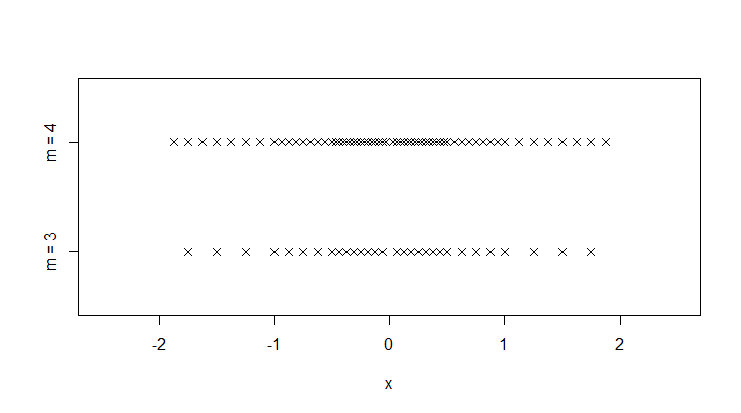
\includegraphics[height = 4.5cm, width = 8.5cm]{figure_man/Distance.png}
\end{figure}
\end{center}
%<<echo = FALSE, out.width="0.7\\textwidth">>=
%e = -1:1
%x = list()
%k = 1
%for(j in 3:4) {
%  x[[k]] = NA
%  u = expand.grid(rep(list(0:1), length = j))
%  for(i in 1:length(e)) {
%    for(ii in 1:nrow(u)) {
%      tx = 2^e[i] * sum(u[ii, ] * 2^(1:j * -1))
%      x[[k]] = c(x[[k]], tx, -1 * tx)
%    }
%  }
%  x[[k]] = x[[k]][x[[k]] != 0]
%  k = k + 1
%}

%plot(x[[1]], rep(1, length(x[[1]])), ylim = c(0.5, 2.5), xlim = c(-2.5, 2.5),
%  axes = FALSE, xlab = "x", ylab = "", pch = 4)
%axis(2, at = c(1, 2), labels = c("m = 3", "m = 4"))
%points(x[[2]], rep(2, length(x[[2]])), pch = 4)
%axis(1)
%box()
%@


\framebreak

The distance between the representable numbers is important:
\begin{itemize}
 \item The smallest numbers around $0$ are $\pm b^{e_{\min}-m}$. \\[2mm]
 \item The smallest number greater than $1$ is $1+b^{-m}$ \\
 ($e = 0$, $u_0 = \hdots = u_{m-1} = 0$ and $u_m = 1$). \\[2mm]
  % $$
  % 1 = 2^1 \cdot \left(1/2 + \sum_{i = 2}^m 0 \cdot 2^{-i}\right) \rightarrow 2^1 \cdot 2^{-1} + 2^1 \cdot 2^{-m} = 1 + 2^{1 - m}
  % $$
 \item The largest real number less than $1$ is $1-b^{-m-1}$ \\
 ($e = -1, u_0 = 0$ and $u_1 = \hdots = u_m = 1$). \\[2mm]
 \item This results in important constants called
  "machine epsilons":
  $$
    \label{eq:2}
    \epsilon_{\min} = b^{-m-1} \qquad % https://en.wikibooks.org/wiki/Floating_Point/Epsilon
    \epsilon_{\max} = b^{-m}
  $$
 \item For numbers greater than $b^{m + 1}$, the distance between numbers is $> 1$ and even integer parts
   are no longer exact.

\end{itemize}

\framebreak

Machine epsilons can be used to estimate the distance between the
numbers in the entire domain.

\lz

In general: Around a number $x\ne 0$, the \textbf{relative distance} between machine numbers is approximately \textbf{$\epsilon_{\max}$}, and
the \textbf{absolute distance} is thus \textbf{$x\cdot\epsilon_{\max}$}
(approximately, since neither $x$ nor the product with $\epsilon_{\max}$
need to be representable).

\lz

The estimate with $\epsilon_{\max}$ is conservative and therefore
usually preferred.

\lz

From now on, we define
$\epsm := \epsilon_{\max}$.

\lz

This machine epsilon is our minimal accuracy.


% \framebreak

% o.B.d.A. sei $x\ge 0$, $b^{e-1}\le x< b^e$, und die
% Gleitkommadarstellung
% $$
%   \xt = b^e \sum_{i=1}^m u_i b^{-i}
% $$
% Der absolute Abstand zweier Maschinenzahlen im Intervall
% $[b^{e-1},b^e]$ ist $b^{e-m}$, daher ist der absolute Fehler betragsmäßig
% $$
%   |\xt - x| \le b^{e-m}
% $$
% sowie der relative Fehler betragsmäßig
% $$
% \frac{|\xt - x|}{x} \le \frac{b^{e-m}}{x}
%   \le \frac{b^{e-m}}{b^{e-1}} = b^{1-m} = \epsm
% $$
% Allgemein gilt daher
% $ \qquad \qquad
%   |\xt - x| \le \epsm |x|
% $ \\  Bei Rundung gewinnt man noch einen Faktor 1/2.

\framebreak
\lz
\begin{verbatim}
options(digits = 20)
1 + 1 / (2^53)
## [1] 1
\end{verbatim}

\vspace{0.3cm}
\begin{verbatim}
1 + 1 / (2^52)
## [1] 1.0000000000000002
\end{verbatim}

\vspace{0.3cm}
\begin{verbatim}
1 / (2^52)
## [1] 2.2204460492503131e-16
\end{verbatim}

\vspace{0.3cm}
\begin{verbatim}
.Machine$double.eps
## [1] 2.2204460492503131e-16
\end{verbatim}


\end{vbframe}

\endlecture
\end{document}

% https://github.com/SurajGupta/r-source/blob/56becd21c75d104bfec829f9c23baa2e144869a2/src/library/stats/src/cov.c

